\begin{flushright} {\tiny {\color{gray} basis\_Q3\_2D.tex}} \end{flushright}
%~~~~~~~~~~~~~~~~~~~~~~~~~~~~~~~~~~~~~~~~~~~~~~~~~~~~~~~~~~~~~~~~~~~~~~~~~~~~~~~~~~~~~~~~~~~~~~~~~~

Inside an element the local numbering of the nodes is as follows:

\begin{flushright} {\tiny {\color{gray} (tikz\_q32d.tex)}} \end{flushright}
%~~~~~~~~~~~~~~~~~~~~~~~~~~~~~~~~~~~~~~~~~~~~~~~~~~~~~~~~~~~~~~~~~~~~~~~~~~~~~~~~~~~~~~~~~~~~~~~~~~


\begin{center}
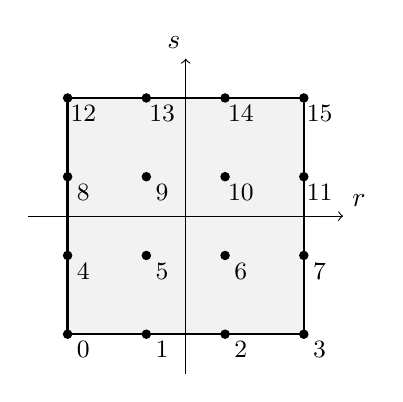
\begin{tikzpicture}
%\draw[step=0.5cm,gray,very thin] (0,0) grid (5,5); 
\draw[fill=gray!10,gray!10](1,1) rectangle (4,4);
\draw[thick] (1,1)--(4,1)--(4,4)--(1,4)--cycle;
\draw [->] (0.5,2.5) -- (4.5,2.5);
\draw [->] (2.5,0.5) -- (2.5,4.5);
\node[] at (4.7,2.7) {$r$};
\node[] at (2.35,4.7) {$s$};
\draw[black,fill=black] (1,1)   circle (1.5pt);
\draw[black,fill=black] (1,2)   circle (1.5pt);
\draw[black,fill=black] (1,3)   circle (1.5pt);
\draw[black,fill=black] (1,4)   circle (1.5pt);
\draw[black,fill=black] (2,1)   circle (1.5pt);
\draw[black,fill=black] (2,2)   circle (1.5pt);
\draw[black,fill=black] (2,3)   circle (1.5pt);
\draw[black,fill=black] (2,4)   circle (1.5pt);
\draw[black,fill=black] (3,1)   circle (1.5pt);
\draw[black,fill=black] (3,2)   circle (1.5pt);
\draw[black,fill=black] (3,3)   circle (1.5pt);
\draw[black,fill=black] (3,4)   circle (1.5pt);
\draw[black,fill=black] (4,1)   circle (1.5pt);
\draw[black,fill=black] (4,2)   circle (1.5pt);
\draw[black,fill=black] (4,3)   circle (1.5pt);
\draw[black,fill=black] (4,4)   circle (1.5pt);
\node[] at (1.2,0.8) {\small $0$};
\node[] at (2.2,0.8) {\small $1$};
\node[] at (3.2,0.8) {\small $2$};
\node[] at (4.2,0.8) {\small $3$};
\node[] at (1.2,1.8) {\small $4$};
\node[] at (2.2,1.8) {\small $5$};
\node[] at (3.2,1.8) {\small $6$};
\node[] at (4.2,1.8) {\small $7$};
\node[] at (1.2,2.8) {\small $8$};
\node[] at (2.2,2.8) {\small $9$};
\node[] at (3.2,2.8) {\small $10$};
\node[] at (4.2,2.8) {\small $11$};
\node[] at (1.2,3.8) {\small $12$};
\node[] at (2.2,3.8) {\small $13$};
\node[] at (3.2,3.8) {\small $14$};
\node[] at (4.2,3.8) {\small $15$};
\end{tikzpicture}
\end{center}



The 1D cubic basis functions are given by:
\begin{align}
\bN_1(r)&=(-1   +r +9r^2 - 9r^3)/16 & \bN_1(t)&=(-1   +t +9t^2 - 9t^3)/16 \nonumber\\
\bN_2(r)&=(+9 -27r -9r^2 +27r^3)/16 & \bN_2(t)&=(+9 -27t -9t^2 +27t^3)/16 \nonumber\\
\bN_3(r)&=(+9 +27r -9r^2 -27r^3)/16 & \bN_3(t)&=(+9 +27t -9t^2 -27t^3)/16 \nonumber\\
\bN_4(r)&=(-1   -r +9r^2 + 9r^3)/16 & \bN_4(t)&=(-1   -t +9t^2 + 9t^3)/16 \nonumber
\end{align}

The resulting basis functions are simply the tensor product of the above 1D ones:

\begin{mdframed}[backgroundcolor=blue!5]
\begin{eqnarray}
\bN_{01}(r,s)&=&\bN_1(r)\bN_1(s) = (-1   +r +9r^2 - 9r^3)/16 \cdot (-1  +t +9s^2 - 9s^3)/16 \nonumber\\
\bN_{02}(r,s)&=&\bN_2(r)\bN_1(s) = (+9 -27r -9r^2 +27r^3)/16 \cdot (-1  +t +9s^2 - 9s^3)/16 \nonumber\\
\bN_{03}(r,s)&=&\bN_3(r)\bN_1(s) = (+9 +27r -9r^2 -27r^3)/16 \cdot (-1  +t +9s^2 - 9s^3)/16 \nonumber\\
\bN_{04}(r,s)&=&\bN_4(r)\bN_1(s) = (-1   -r +9r^2 + 9r^3)/16 \cdot (-1  +t +9s^2 - 9s^3)/16 \nonumber\\
\bN_{05}(r,s)&=&\bN_1(r)\bN_2(s) = (-1   +r +9r^2 - 9r^3)/16 \cdot (9 -27s -9s^2 +27s^3)/16 \nonumber\\
\bN_{06}(r,s)&=&\bN_2(r)\bN_2(s) = (+9 -27r -9r^2 +27r^3)/16 \cdot (9 -27s -9s^2 +27s^3)/16 \nonumber\\
\bN_{07}(r,s)&=&\bN_3(r)\bN_2(s) = (+9 +27r -9r^2 -27r^3)/16 \cdot (9 -27s -9s^2 +27s^3)/16 \nonumber\\
\bN_{08}(r,s)&=&\bN_4(r)\bN_2(s) = (-1   -r +9r^2 + 9r^3)/16 \cdot (9 -27s -9s^2 +27s^3)/16 \nonumber\\
\bN_{09}(r,s)&=&\bN_1(r)\bN_3(s) = (-1   +r +9r^2 - 9r^3)/16 \cdot (9 +27t -9t^2 -27t^3)/16 \nn\\
\bN_{10}(r,s)&=&\bN_2(r)\bN_3(s) = (+9 -27r -9r^2 +27r^3)/16 \cdot (9 +27t -9t^2 -27t^3)/16 \nn\\
\bN_{11}(r,s)&=&\bN_3(r)\bN_3(s) = (+9 +27r -9r^2 -27r^3)/16 \cdot (9 +27t -9t^2 -27t^3)/16 \nn\\
\bN_{12}(r,s)&=&\bN_4(r)\bN_3(s) = (-1   -r +9r^2 + 9r^3)/16 \cdot (9 +27t -9t^2 -27t^3)/16 \nn\\
\bN_{13}(r,s)&=&\bN_1(r)\bN_4(s) = (-1   +r +9r^2 - 9r^3)/16 \cdot (-1   -t +9t^2 + 9t^3)/16\nn\\
\bN_{14}(r,s)&=&\bN_2(r)\bN_4(s) = (+9 -27r -9r^2 +27r^3)/16 \cdot (-1   -t +9t^2 + 9t^3)/16\nn\\
\bN_{15}(r,s)&=&\bN_3(r)\bN_4(s) = (+9 +27r -9r^2 -27r^3)/16 \cdot (-1   -t +9t^2 + 9t^3)/16\nn\\
\bN_{16}(r,s)&=&\bN_4(r)\bN_4(s) = (-1   -r +9r^2 + 9r^3)/16 \cdot (-1   -t +9t^2 + 9t^3)/16
\end{eqnarray}
\end{mdframed}

\todo[inline]{produce derivatives}

These basis functions are used in \stone 19.



